\newpage
\part{Monte Carlo Tree Search}
\section{Description de l'algorithme}
L'algorithme Monte Carlo Tree Search est un algorithme de recherche heuristique qui explore intelligemment l'arbre des actions possibles à partir de l'état courant du jeu et ce, jusqu'à ce que toutes les configurations du jeu soient explorées. Cet algorithme choisit en priorité les branches qui sont le plus susceptibles de mener à une victoire. Il maintient par ailleurs un compromis entre l'exploitation et exploration en utilisant l'algorithme UCB pour choisir la prochaine branche à explorer en priorité. 
\section{Implémentation}
Nous avons implémenté cet algorithme à l'aide de trois classes, à savoir \verb@State_Move@, \verb@UCTree@ et \verb@UCTPlayer@. La première représente un couple état-coup, i.e.\ un n\oe ud dans l'arbre de décision. Par ailleurs, \verb@UCTree@ est l'implémentation de cet algorithme à proprement parler car elle contient toutes les fonctionnalités nécessaires à son utilisation. Enfin, \verb@UCPlayer@ correspond au joueur \verb@UCT@. En effet, il hérite de \verb@Agent@ et implémente la méthode \verb@get_action@ dans laquelle il crée un arbre enraciné à l'état courant du jeu et puis, pour $N$ itérations, il simule une partie entre deux joueurs aléatoires et utilise la séquence de coups obtenue pour mettre à jour son arbre de décision en stockant le premier couple état-coup pas encore présent dans l'arbre. La méthode renvoie l'action avec la plus grande récompense.

\section{Mise en oeuvre}
\begin{figure}[!h]
\centering
  \begin{center}
    \subfloat[Espérance de gain contre le joueur $Random$ lorsqu'il entame les parties][Espérance de gain contre le joueur $Random$ lorsqu'il entame les parties]{
      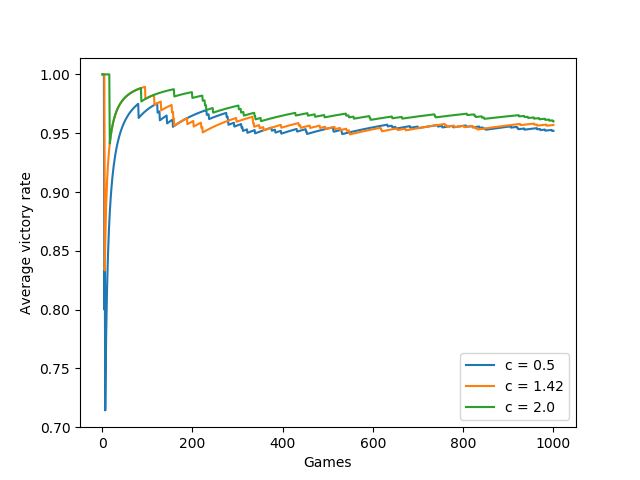
\includegraphics[width=0.5\textwidth]{Project_1/Report/sections/Figures/uct_first_rand.png}
      \label{sub:}
                         }
    \subfloat[Espérance de gain contre le joueur $Random$ lorsque ce dernier entame les parties]{
      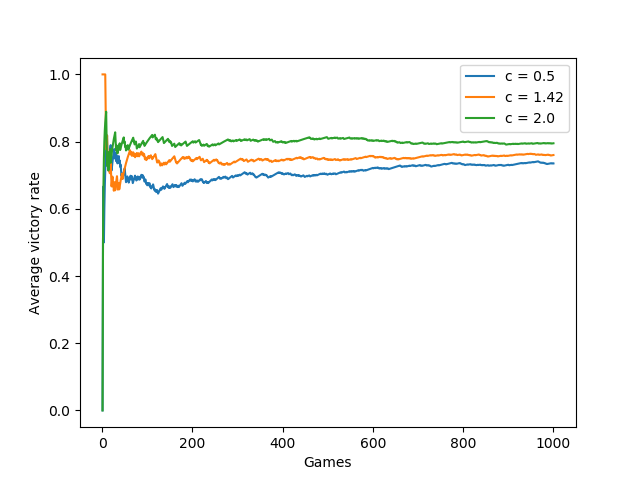
\includegraphics[width=0.5\textwidth]{Project_1/Report/sections/Figures/uct_last_rand.png}
      \label{sub:s}
                          }
    \newline
    \subfloat[Espérance de gain contre le joueur $Monte$ $Carlo$ lorsqu'il entame les parties]{
      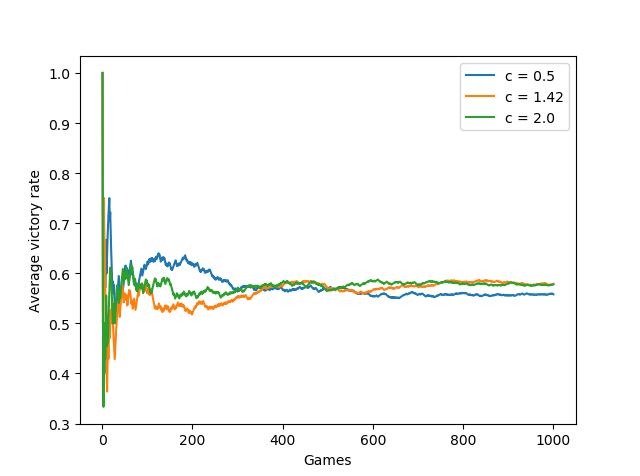
\includegraphics[width=0.5\textwidth]{Project_1/Report/sections/Figures/uct_first_mc.png}      \label{sub:}
                         }
    \subfloat[Espérance de gain contre le joueur $Monte$ $Carlo$ lorsque ce dernier entame les parties]{
      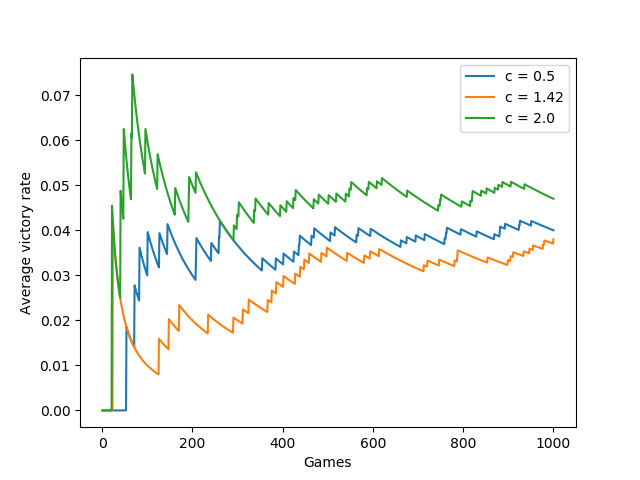
\includegraphics[width=0.5\textwidth]{Project_1/Report/sections/Figures/uct_last_mc.png}
      \label{sub:s}
                          }
    \caption[Benchmark du joueur UCT]{Comparaison entre un joueur $UCT$, avec un nombre d'échantillonnages égal à 100, et les joueurs $Random$ et $Monte$ $Carlo$}
    \label{fig:renonculacees}
  \end{center}
\end{figure}

Dans la figure 7, de la même manière que dans la section 6, le joueur UCT est largement plus intelligent que le joueur aléatoire et ses résultats sont atténués lorsqu'il affronte le joueur Monte Carlo.

Par ailleurs, nous y voyons aussi que la répercussion du paramètre $c$ modulant l'équilibre entre l'exploration et l'exploitation sur les performances de l'algorithme UCT est moindre. En effet, le joueur UCT effectue plus d'exploitation en raison de sa formule qui privilégie les meilleurs coups à différence du joueur $Monte$ $Carlo$ qui explore beaucoup plus de résultats possibles.

C'est ce manque d'exploration qui explique les mauvais résultats du joueur UCT lorsqu'il joue en deuxième vis-à-vis du joueur $Monte$ $Carlo$.